\documentclass[12pt,titlepage]{article}
\usepackage{graphicx}
\author{The TOME Team}
\title{\textbf{TOME Application Model}}
\begin{document}
\maketitle
\tableofcontents
\listoffigures
\newpage
\section{Introduction}
\subsection{Purpose of Document}
The purpose of this document is to specify the TOME system and the application model it uses.
\subsection{Background}
In December of 2003, several students on Dorm 41 started a system called TOME.  The basic idea is that at the end of the semester, instead of everyone selling their books back to the bookstore, they all donate them to central repository.  Anyone on the floor can then check out whatever books they need free of charge for a semester.

The advantage of having a computer-based system to keep track of all those books is easy to see, and one has been under development ever since the start of TOME.  Since its humble beginnings as a quick solution over Christmas break, the system has grown to well over 3,000 lines of Perl code as well as HTML templates, a well-planned database schema, and significant documentation.  The system not only has comprehensive facilities for tracking books and patrons, but also keeps tabs on what books are used for what classes and other alternatives to purchasing new books.
\subsection{References}
All project data will be stored in a combination Subversion repository and Trac environment.  All of this will be made viewable at the following URL:

\texttt{http://enosh.letnet.net/trac/tome}
\section{Application Overview}
\subsection{Scope}
The TOME system is responsible for managing:
\begin{itemize}
	\item Books
	\item Book information
	\item Class information
	\item Class-to-book mappings
	\item Book reservations
	\item Book checkouts
\end{itemize}
The TOME system is \textbf{not} responsible for managing:
\begin{itemize}
	\item Book acquisition
	\item Book disposal
	\item Selling old books
	\item Any financial activity
\end{itemize}
\subsection{Context}
TOME exists as an independent system with no ties to other databases.  Information from other databases, such as class listings, book information, and book-to-class associations will be used, but not in an automated fashion.
\subsection{Technical Environment}
TOME is a web-based Perl application.  It is intended to be run under the Apache webserver, but any webserver that supports CGI should be capable of running the system.  Template::Toolkit is used to process HTML templates.  PostgreSQL is used as the database backend.  CGI::Application is used as the framework for the system as a whole.
\section{Actors}
\subsection{Actor Diagram}
Figure~\ref{userdiagram} shows an overview of the actors involved in the TOME system and how they interact with each other.  Patrons talk to TOMEkeepers who use the TOME web interface which is based on the TOME database.
\begin{figure}[h]
	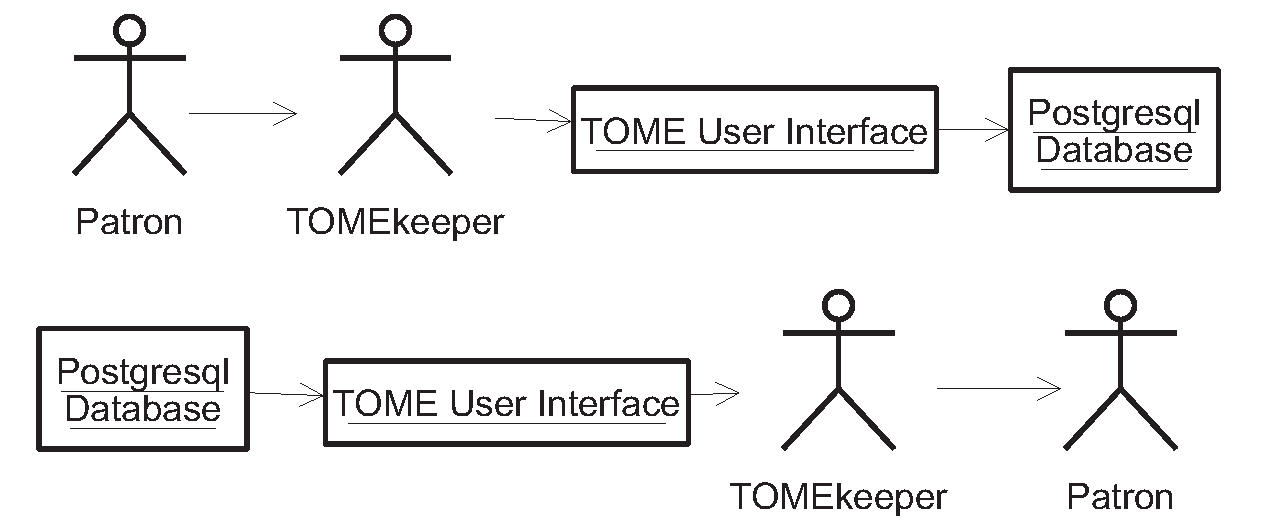
\includegraphics[width=\textwidth]{userdiagram}
	\caption{Actor Diagram}
	\label{userdiagram}
\end{figure}
\subsection{Actor Definitions}

\subsubsection{Patron}
\begin{tabular}{|p{.25\textwidth}|p{.75\textwidth}|}
	\hline
	\textbf{Description} & The Patron is any student who wishes to use the TOME system.  Only students that reside on floors with an active TOME system can become Patrons. Patrons never interact directly with TOME, only through TOMEkeepers.  \\
	\hline
	\textbf{Aliases} & Student. \\
	\hline
	\textbf{Inherits} & None. \\
	\hline
	\textbf{Actor Type} & Passive - Person. \\
	\hline
\end{tabular}

\subsubsection{TOMEkeeper}
\begin{tabular}{|p{.25\textwidth}|p{.75\textwidth}|}
	\hline
	\textbf{Description} & The TOMEkeeper is the primary user of the TOME system.  They are responsible for all interactions with Patrons, all system administration, and all TOME activity. \\
	\hline
	\textbf{Aliases} & None. \\
	\hline
	\textbf{Inherits} & None. \\
	\hline
	\textbf{Actor Type} & Active - Person. \\
	\hline
\end{tabular}

\section{Business Use Cases}
\subsection{Use Case Listing}
\begin{tabular}{|p{.10\textwidth}|p{.40\textwidth}|p{.50\textwidth}|}
	\hline
	\textbf{ID} & \textbf{Use Case Name} & \textbf{Comments} \\
	\hline
	UC01 & Book Added & testing 1 2 3 \\
	\hline
\end{tabular}
\subsection{Graphical Use Case Diagram}
\begin{figure}[h]
	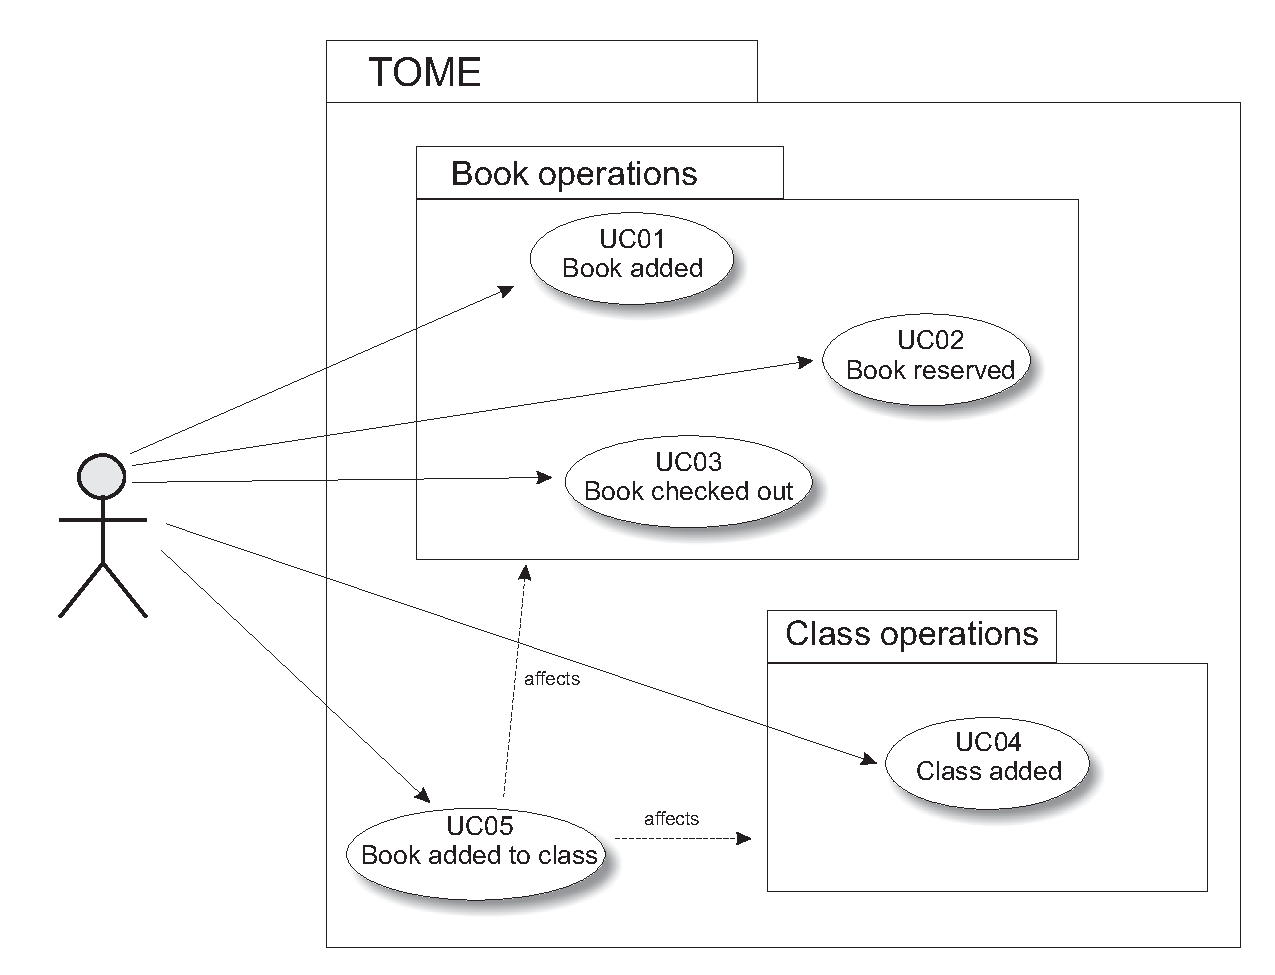
\includegraphics[width=\textwidth]{GraphicalUseCaseDiagram}
	\caption{Use Case Diagram}
	\label{usecase}
\end{figure}
\subsection{Business Use Cases}
This section documents the complete business scenarios within the scope of this project.
\subsubsection{UC01: Book Added}
\paragraph{Description}
test

\section{Database Structure}
The overall structure of the database can be seen in Figure~\ref{tomedb}.  In addition to the structure, there are also triggers that ensure the consistency of the database at all times.
\begin{figure}[h]
	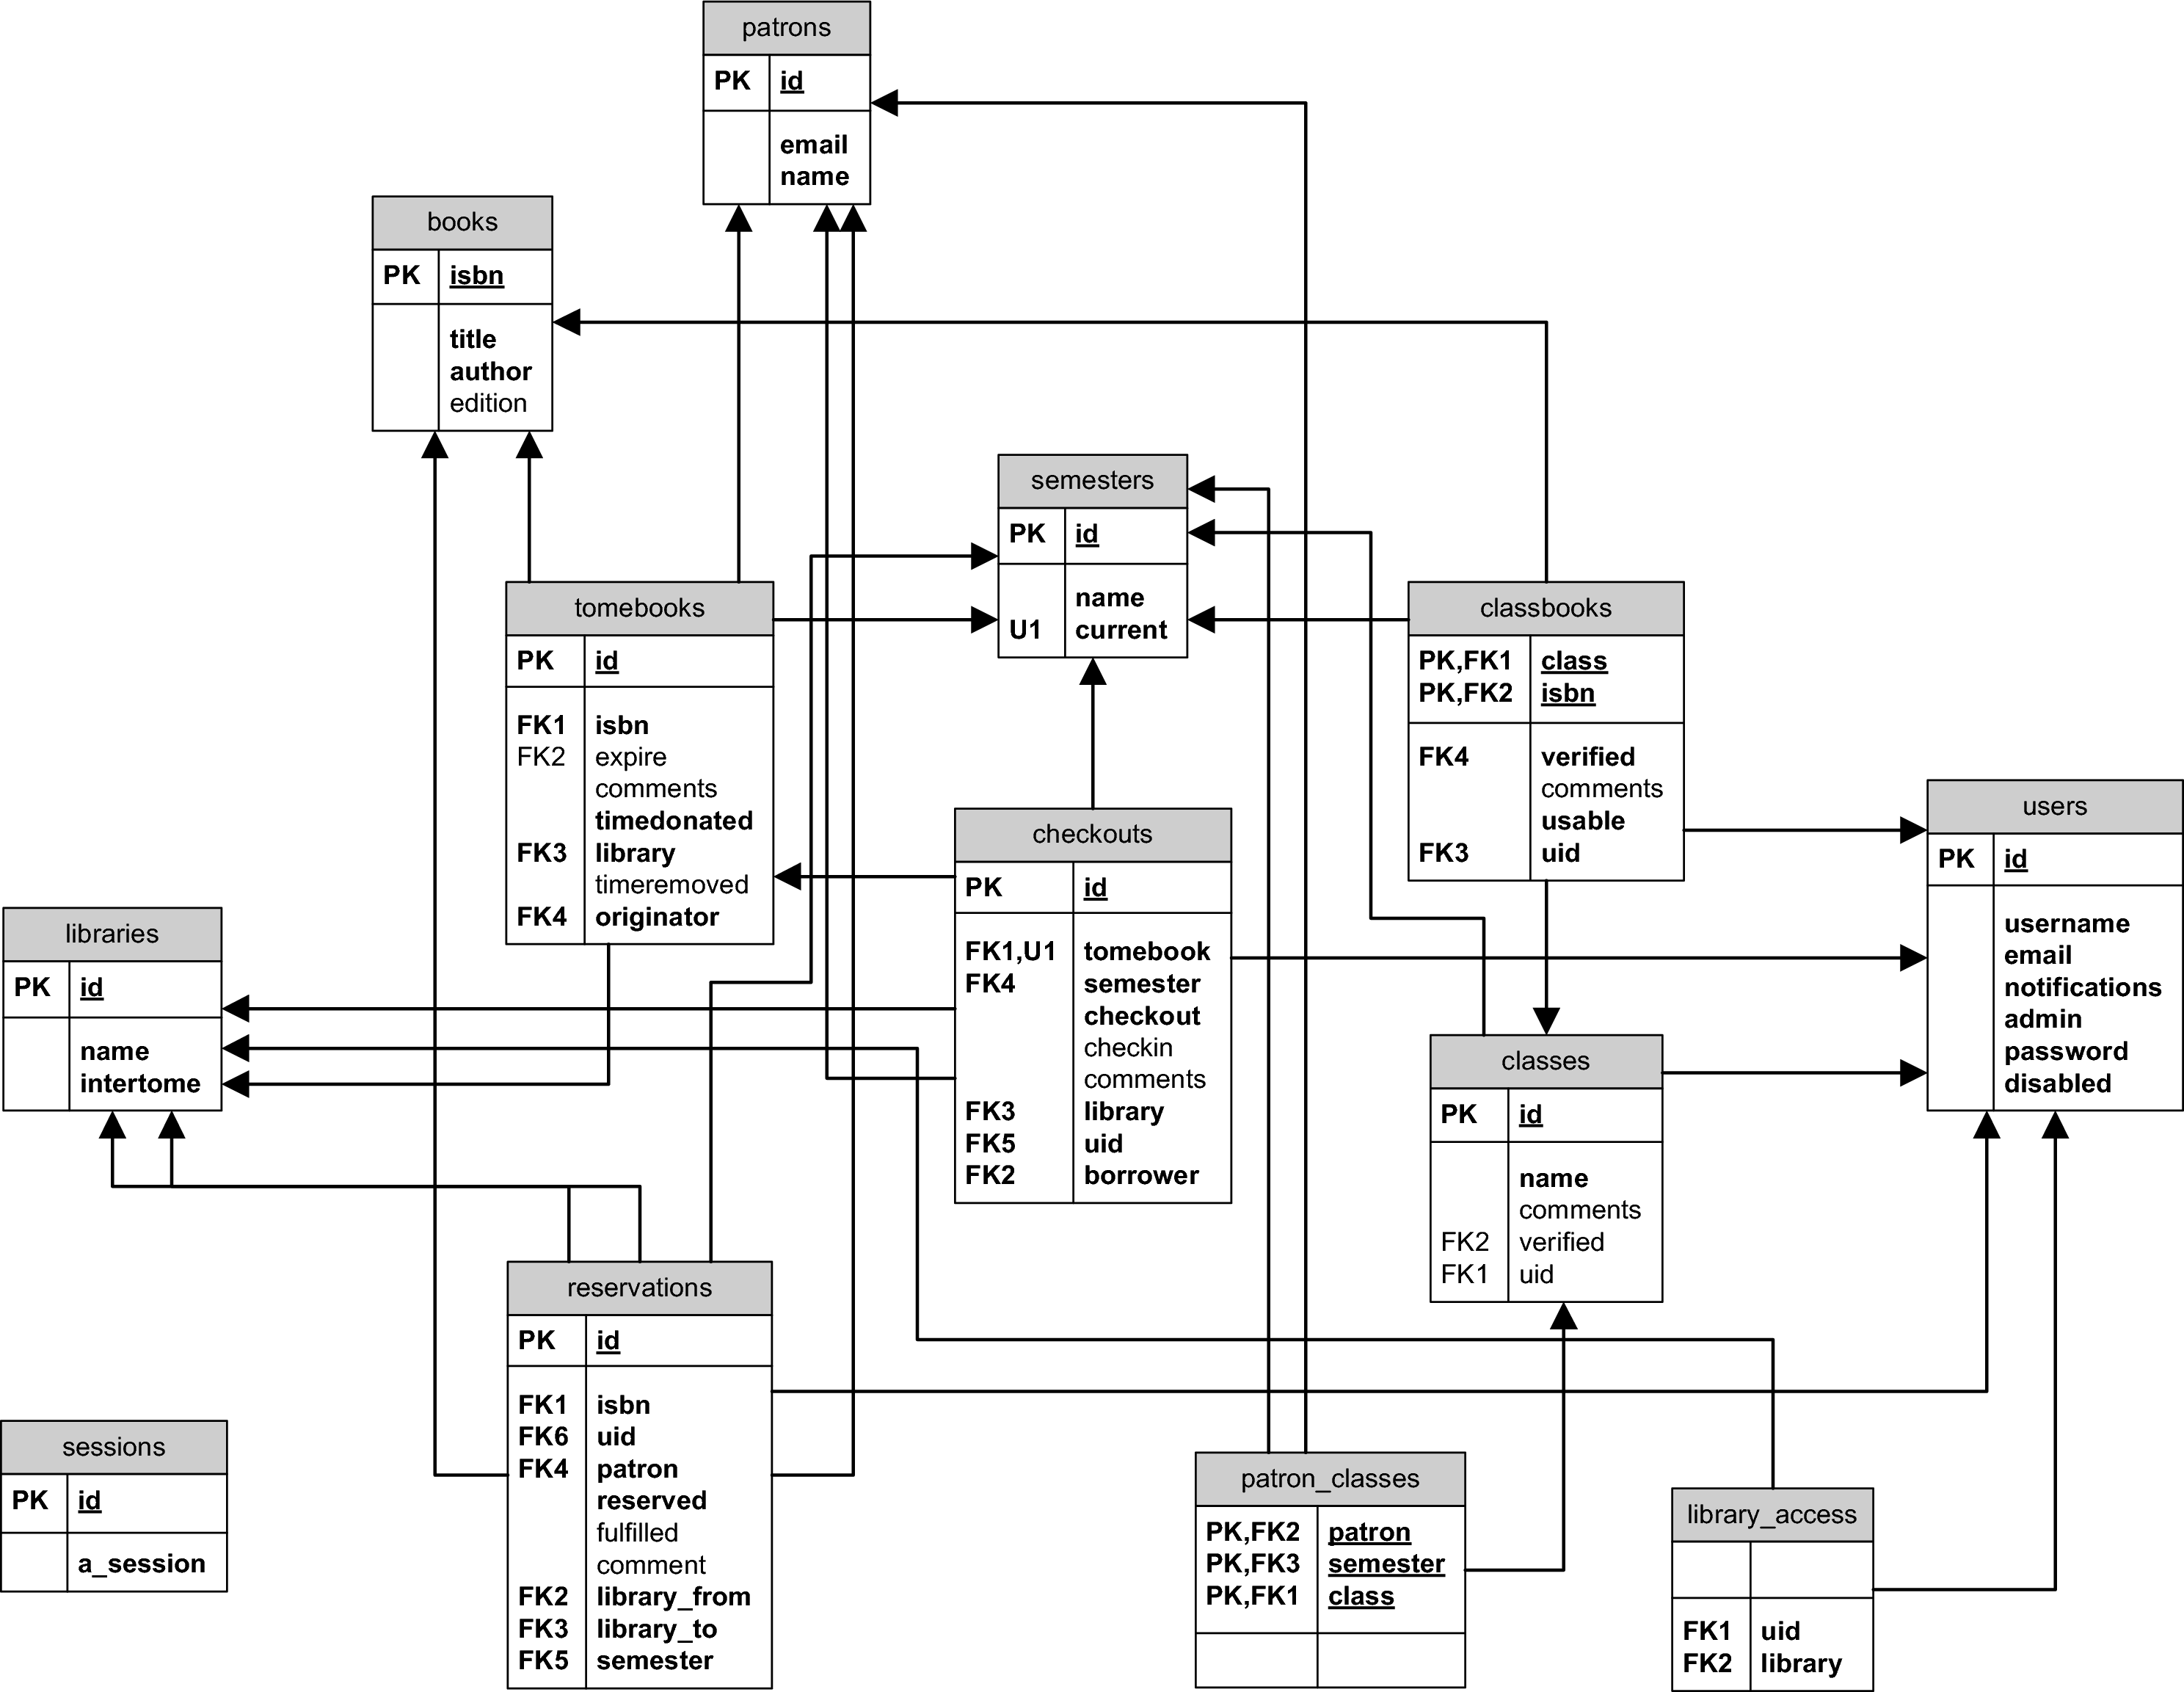
\includegraphics[width=\textwidth]{tomedb}
	\caption{Database Diagram}
	\label{tomedb}
\end{figure}
\end{document}

